% Versión 2023
%

% la section y label cargado en el archivo madre

% \section{Buses de Datos en Avi\'onica}
% \label{sec:U01.05.buses.datos.avionica}

    Las se\~nales que se env\'ian entre los distintos componentes del
    EIS se transmiten por una l\'inea de transmisi\'on digital
    denominada ``{\it Bus de Datos}". Las se\~nales transmitidas son
    peque\~nos pulsos de tensi\'on en c\'odigo binario (unos y
    ceros). Seg\'un el protocolo, los unos y ceros se diferencian por
    tener valores distintos de tensiones positivas o negativas,
    variaciones de tensiones ascendentes o descendentes, falta de
    tensi\'on, etc. Los pusos de tensi\'on tienen duraciones
    extremadamente breves a fin de enviar una gran cantidad de
    informaci\'on en poco tiempo.

Estos son los pilares de los modernos sistemas de avi\'onica integrados, permitiendo el intercambio
de informaci\'on entre los diferentes sistemas de la aeronave. Transmiten la informaci\'on para
los datos de ingreso en un sistema y comunican los resultados para otros usuarios.

La palabra ``\emph{bus}'' es una contracción de la palabra griega ``\emph{ómnibus}'' cuyo significado es  ``\emph{para todos}''. Por lo tanto, en el contexto de computadoras y sistemas digitales, ``\emph{bus}'' se refiere a un sistema que permite la interconexión y el intercambio de datos entre los dispositivos en un sistema complejo. Sin embargo, se debe tener en cuenta que la ``\emph{interconexión}'' implica algo más que un cableado físico puesto que, entre otras cosas, define los niveles de tensión  y las reglas (o protocolos) que rigen la transferencia de datos.

Con una cantidad tan grande de sistemas de aviónica, una aeronave moderna requiere una cantidad considerable de cableado. Además, algunos de estos tendidos en una aeronave grande pueden tener una longitud considerable.

 \begin{myboxVerde}{\bf ¿C\'omo ahorrar peso? }
Con el correr de los años y los avances realizados en aviónica y sistemas de las aeronaves, estos se incrementan en las mismas y la comunicación entre ellos se vuelve más compleja. 

Por otra parte el cableado de una aeronave equivale a una proporción significativa de su peso sin carga y, por lo tanto, minimizar la cantidad de cableado  es una consideración importante en el diseño de aeronaves modernas, tanto civiles como militares.

\begin{minipage}[c]{0.3\linewidth}
  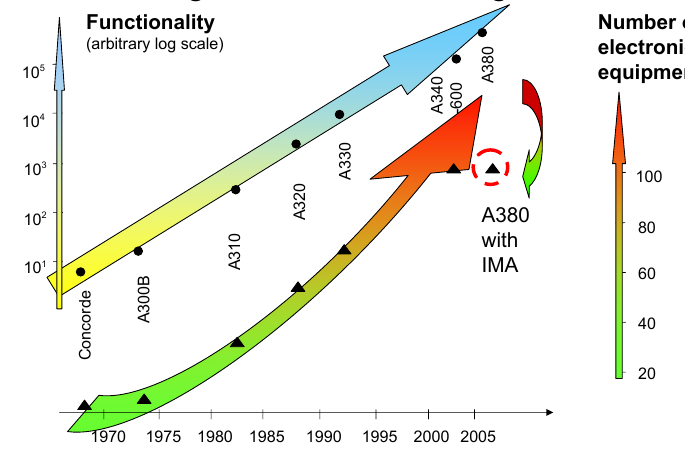
\includegraphics[width=\linewidth]{01.tablero.instrumentos/imagenes/1.5.protocolos.buses.datos/7-A380-IMA.png}
  \captionof{figure}{Aumento de sistemas de aviónica en el tiempo
   \protect\cite{a380IMA}}
\end{minipage}\hspace{1.5em}
\begin{minipage}[c]{0.3\linewidth}
  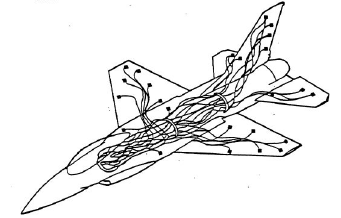
\includegraphics[width=\linewidth]{01.tablero.instrumentos/imagenes/1.5.protocolos.buses.datos/8-avion+cableado.png}
  \captionof{figure}{Conexiones punto a punto  \protect\cite{MIL-1553-tutorial} }
\end{minipage}\hspace{1.5em}
\begin{minipage}[c]{0.3\linewidth}
  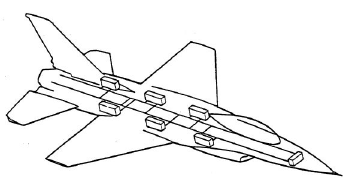
\includegraphics[width=\linewidth]{01.tablero.instrumentos/imagenes/1.5.protocolos.buses.datos/9-avio+arquitectura+bus.png}
  \captionof{figure}{Conexiones con bus de datos \protect\cite{MIL-1553-tutorial} }
\end{minipage}

\end{myboxVerde}




\subsection{Conceptos generales}
\label{sec:01.05.01.01.conceptos.generales.buses}

Los sistemas de bus pueden ser unidireccionales  o bidireccionales, como se muestra en la Figura \ref{fig:01.sistemas.bus.datos}. 
También pueden ser seriales (un \ac{Bit} de datos transmitido a la vez) o paralelos (donde a menudo aparecen 8, 16 o 32 bits de datos como un grupo en varias líneas de datos transmitido al mismo tiempo). Debido a las restricciones impuestas por la longitud y el peso del conductor, todos los sistemas prácticos de bus de datos en aeronaves se basan en la transferencia de datos en serie en lugar de en paralelo.

\begin{figure}[!htb]
  \centering
  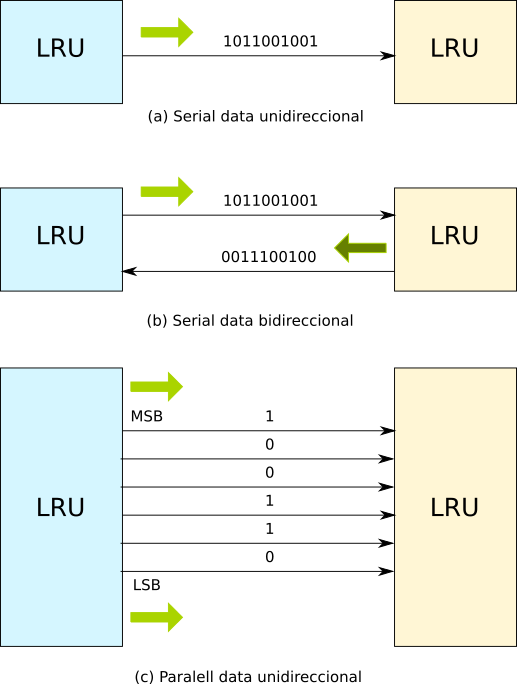
\includegraphics[width=0.4\textwidth]{01.tablero.instrumentos/U01.imagenes/U01.5.protocolos.buses.datos/01_Uni_bi_paralelo_datos.png}
  \caption{Sistemas de bus de datos. Adaptado de \protect\cite{tooley2013aircraft}}
  \label{fig:01.sistemas.bus.datos}
\end{figure}


Los sistemas de bus proporcionan un medio eficiente para intercambiar datos entre los diversos sistemas de aviónica que se encuentran en una aeronave moderna.
Las Unidades Reemplazables de Línea, en ingl\'es  \ac{LRU}, como la interfaz de datos del motor o las unidades electrónicas de flaps/slats están conectadas al bus por medio de un acoplador de bus dedicado y un módulo de interfaz en serie.

Dentro de la \ac{LRU}, la lógica digital dedicada y los sistemas de microprocesador que procesan datos localmente utilizan cada uno su propio sistema de bus local los cuales emplean, invariablemente, la transferencia de datos en paralelo que resulta ideal para mover grandes cantidades de datos muy rápidamente pero solo durante distancias cortas.

Teniendo en cuenta la temporización los buses se dividen en:
\begin{description}
\item[Síncronos] requieren de un reloj en sus líneas de control, todos los equipos trabajan con la misma velocidad.
\item[Asíncronos] requieren un ``{\it \bf handshaking}'', mediante el cual los equipos que necesitan comunicarse se ponen de acuerdo previamente.

\end{description}

Respecto a la velocidad de transmisión se tienen:

\begin{description}
\item[LS channel] o canal de baja velocidad, usualmente de cobre.
\item[HS channel] o canal de alta velocidad, de fibra óptica.
\end{description}

%PUNTO CLAVE

\begin{tcolorbox}
  Las aeronaves modernas utilizan múltiples sistemas de bus de forma
  redundante para intercambiar datos entre los diversos sistemas y
  subsistemas de aviónica. Estos sistemas de bus utilizan la
  transferencia de datos en serie porque minimiza el tamaño y el peso
  del cableado de la aeronave.
\end{tcolorbox}

\subsection{Protocolos de bus}
\label{sec:01.05.01.02.protocolos.bus}


La noción de un protocolo necesita una pequeña explicación:

Imagine por un momento que se enfrenta con el problema de organizar una discusión entre una gran cantidad de personas sentadas alrededor de una mesa, todas las cuales están con los ojos vendados y, por lo tanto, no pueden verse.

Para asegurarse de que no todos hablen a la vez debe establecer algunas reglas básicas, incluida la forma en que los participantes indican que tienen algo que decir y establecer algunas prioridades sobre quién debería hablar. en el caso de que varios participantes indiquen que desean hablar al mismo tiempo.

Estas (y otras) consideraciones formarían un protocolo acordado entre los participantes para llevar a cabo la discusión. El debate debe continuar sin demasiados problemas, siempre que todos en la sala entiendan y estén dispuestos a aceptar el protocolo que se ha establecido. 


Los protocolos de comunicación permiten el intercambio eficiente de datos entre varios dispositivos conectados al mismo bus. Onsisten en un conjunto de reglas y especificaciones que rigen, entre otras cosas, el formato de datos y las conexiones físicas.


% En las computadoras y los sistemas digitales, los protocolos de comunicación se establecen para permitir el intercambio eficiente de datos entre múltiples dispositivos conectados al mismo bus.

 Una serie de estándares diferentes para protocolos se utilizan comúnmente en avi\'onica.
 Respecto a los protocolos actualmente empleados se tiene el ARINC 429, el MIL-STD 1553 y, por ultimo, el AFDX.


% \subsection{Arquitectura del bus}
% \label{sec:01.05.01.03.arquitectura.bus}

% La arquitectura de un bus de datos se refiere a la estructura general de una computadora u otro sistema digital que depende de un bus para su funcionamiento, se describe en forma de un diagrama esquemático de bloques que muestra cómo se interconectan los diversos elementos del sistema y también cómo se organiza el flujo de datos entre los elementos. 

% La arquitectura de un sistema basado en el uso de un sistema de bus serie unidireccional se muestra en la Figura 4.4a, mientras que un sistema de bus bidireccional comparable se muestra en la Figura 4.4b. Pued observarse que el sistema bidireccional simplifica la interconexión de las LRU y permite que todos los dispositivos transmitan y reciban en el mismo bus.





% \subsection{Principios del bus serie}
% \label{sec:01.05.01.04.bus.serie}

% En la Figura 4.5 se muestra un sistema simple para la transferencia de datos en serie entre dos LRU, cada uno de los cuales comprende un sistema aviónico por derecho propio. Dentro de la LRU, los datos se transfieren utilizando un bus de datos paralelo interno (8, 16, 32 o 64 bits de ancho). El enlace entre las dos LRU se realiza utilizando un cable serie simple (a menudo con solo dos, cuatro o seis conductores). La conversión de datos de paralelo a serie y de serie a paralelo se lleva a cabo mediante una interfaz de bus (a menudo se trata de una sola tarjeta o módulo dentro de la LRU). Los datos a transferir pueden ser sincrónicos (utilizando el reloj señales generadas localmente dentro de cada LRU) o pueden ser asíncronas (es decir, auto reloj).

% El sistema que se muestra en la Figura 4.5 tiene la limitación obvia de que los datos solo pueden intercambiarse entre dos dispositivos. En la práctica, necesitamos compartir los datos entre muchas LRU / unidades de aviónica. Esto se puede lograr mediante el sistema de bus ilustrado en la Figura 4.6. En este sistema, los datos se transfieren utilizando un cable de bus de par trenzado blindado, en ingl\'es ``\emph{shielded twisted pair}'',  con una serie de paneles de acoplamiento que se encuentran en los puntos apropiados de la aeronave (por ejemplo, la cubierta de vuelo, la bahía de aviónica, etc.). Cada panel de acoplamiento permite conectar varias unidades de aviónica al bus mediante un cable corto. Para optimizar la velocidad de transferencia de datos y minimizar los problemas asociados con la reflexión y la falta de coincidencia, el cable del bus debe terminarse en cada extremo utilizando un terminador de bus coincidente.

% Los acopladores de bus se producen como unidades de modo de voltaje o de modo de corriente, dependiendo de si usan dispositivos de detección de voltaje o corriente. Dentro de cada unidad LRU / aviónica, se proporciona una interfaz que realiza la conversión de datos de serie a paralelo o de paralelo a serie requerida, como se muestra en la Figura 4.7.

% Además de proporcionar una interfaz eléctrica (con el cambio apropiado de nivel de voltaje y corriente), la unidad de interfaz también convierte los formatos de datos (por ejemplo, de dobletes analógicos en serie presentes en el cable auxiliar a datos en serie codificados por Manchester requeridos por el controlador de terminal), como se muestra en la Figura 4.8. Para transmitir datos utilizando el bus de datos en serie, la información debe presentarse en un formato estándar.

% Un formato típico para datos en serie usaría una longitud de palabra de 32 bits. Esta palabra comprende varios campos discretos, que incluyen:

% \begin{itemize}
%      \item  Hasta 20 bits para datos (que pueden dividirse aún más);

%      \item Un campo de etiqueta de 8 bits que se utiliza para identificar   el tipo de datos y cualquier parámetro que pueda estar asociado a  él.

%      \item Un identificador de origen / destino (SDI);

%      \item Varios bits de estado utilizados para proporcionar informaci\'on   sobre el modo, el estado del hardware o la validez de los datos.

%      \item Un bit de paridad adicional que proporciona un medio para   validar los datos (es decir, determinar si están o no libres de   error).

% \end{itemize}

% PUNTO CLAVE

% Se requiere un medio para convertir los datos en serie en datos paralelos (y viceversa) siempre que una LRU deba conectarse a un sistema de bus de avión.





% Los buses de datos se agrupan en dos conjuntos: 

% \begin{itemize}
%     \item {\bf Simplex} o de un sentido (one way) con un \'unico transmisor y m\'ultiples receptores.
%     \item {\bf Duplex} con m\'ultiples transmisores y receptores.
% \end{itemize}




% En el panorama actual de la aviónica hemos visto pasar un número amplio de
% protocolos que han ido quedando desfasados a lo largo del tiempo. Antes de
% evaluar cada uno de ellos resulta conveniente realizar  un recorrido a la
% importancia de la aviónica en los sistemas de aviación y su evolución.

% Los sistemas han seguido creciendo
% y evolucionando haciendo que sistemas como la comunicación con los
% satélites, sistemas que controlan la electricidad o los sistemas hidráulicos sean
% controlados por electrónica.


\subsubsection{ARINC 429}
\label{sec:01.05.01.ARINC.429}

Creado por \ac{ARINC}, corporación creada en 1929 y compuesta por aerolíneas, fabricantes de aeronaves y de equipos de aviónica. \ac{ARINC} fue creada para producir especificaciones y normas para equipos de aviónica fuera del gobierno para fabricantes nacionales o internacionales.

Es un protocolo utilizado para aviones comerciales y de transporte
y nos cuenta como los equipos de aviónica se comunican unos con otros,
especifica las características eléctricas y de datos.

Se emplea en distintos aviones tanto de Airbus como de Boeing, tal
como A330 o el Boeing 747 o los helicópteros Bell. La fiabilidad de este
protocolo es a costa de un gran peso en cableado y de tasas de envío
limitadas.

El estándar ARINC 429 fue desarrollado a partir del existente estándar ARINC 419, el cual  contiene  especificaciones  de  comunicación  digital  para aviación   comercial.   En   estas   especificaciones   se tienen   cuatro   tipos diferentes  de  topologías  de  cableado,  estando  entre  ellas  una  topología  en serie  que  utiliza  un  par  trenzado  de  cable  apantallado.  Es  esta  topología  en serie la que evolucionó hacia el estándar ARINC 429. 

La primera publicación del ARINC 429 fue en Abril de 1978 y aún existe hoy día bajo  la  nomenclatura  de  ARINC  429-15.  

Este  estándar  está  dividido  en  tres partes:

\begin{description}
\item[Parte 1-15:] Descripción funcional, interfaz eléctrica,
  asignación de etiquetas y formato del paquete de datos.
\item[Parte 2-15:]   Estándares para paquetes de datos discretos. %, define los formatos de paquetes con asignación d.
\item[Parte 3-15:] Técnicas de  transferencias de datos.
\end{description}



ARINC  429  es  un  bus  de  datos   simplex que tiene las siguientes características:

\begin{itemize}
\item Está compuesto por  por dos hilos unidireccionales de datos estándar (puertos Tx y Rx), apantallados y de lazo abierto (open loop) tipo 
Mark 33 Digital Information Transfer System bus.

\item La fuente y el destino deben estar conectados mediante un par de cables trenzados y apantallados. El apantallamiento debe conectarse a masa en ambos lados de la conexión y en todos los conectores intermedios del cableado.

\item Tiene dos velocidades de funcionamiento: baja velocidad entre 12-14,5 Kbps y alta velocidad alcanzando 100 Kbps. 

\item No se pueden utilizar ambas velocidades en el mismo bus.

\item La codificación  es  RZ bipolar

\item El formato de las palabras enviadas por este protocolo es  de  palabras o paquetes de datos  de  32  bits.


\item El protocolo  establece que  debe haber   un   espacio   de   tiempo   entre   cada   palabra (o paquete de datos)   enviada  (GAP).

\item      Las características del mensaje son:
  \begin{itemize}
  \item La información fluye desde una puerta de transmisión hasta una
    o varias puertas de recepción.
  \item En ningún caso la información puede llegar hasta una puerta
    destinada a la transmisión.
  \item La transmisión entre dos LRU en ambos sentidos se
    realiza por buses independientes.
  \end{itemize}

\item El transmisor emite siempre, ya sea 32 bits de datos (palabra) o el estado nulo (NULL).

\item El bus posee un  solo  transmisor  y  hasta  20  receptores.

\item  Si  se  desea implementar  una  comunicación  bidireccional  se  necesitan  dos  canales  o  dos buses.

\end{itemize}


\begin{figure}[!h]
  \centering
%  \scalebox{0.9}{
% ARINC 429 topologias

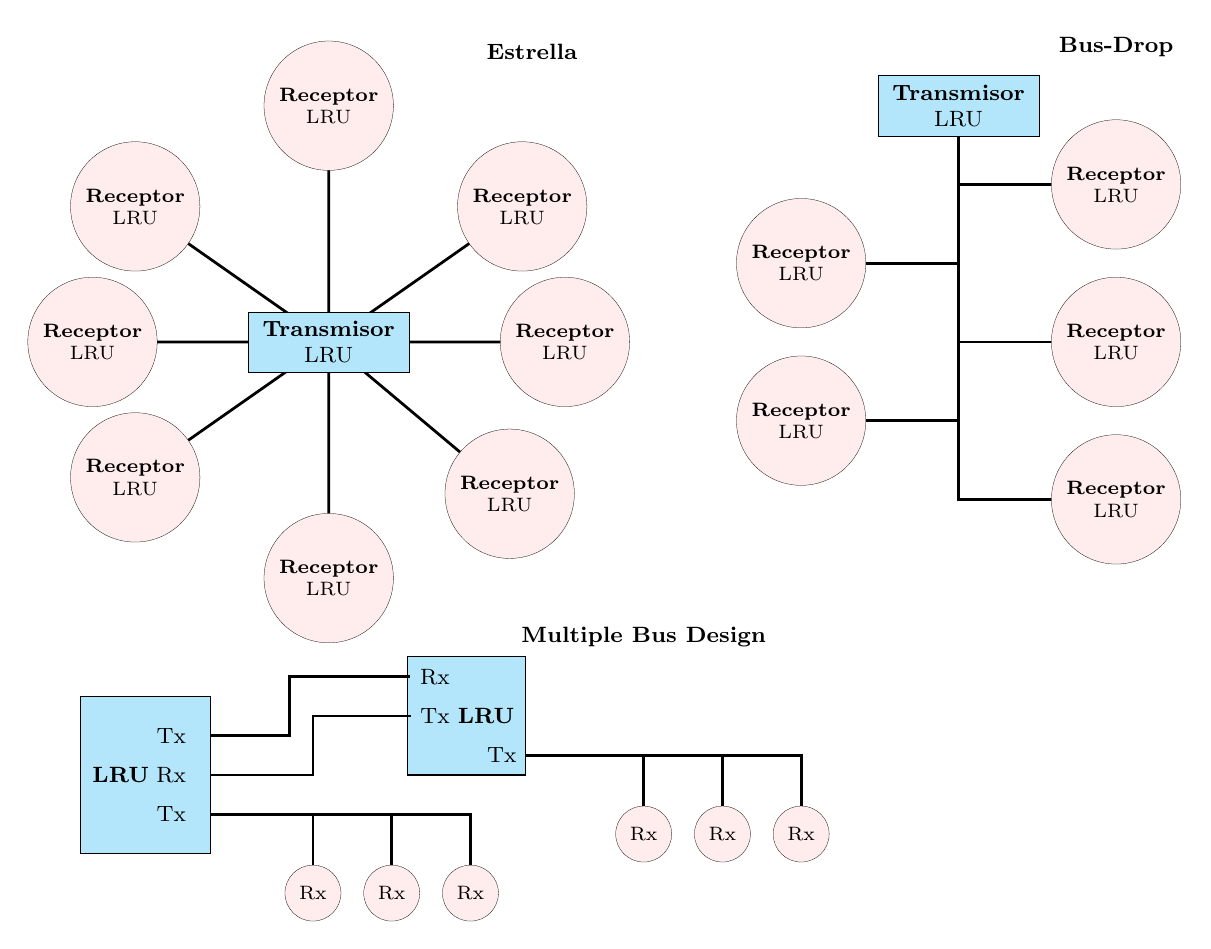
\begin{tikzpicture}[node distance=1cm, 
				font = \footnotesize , 
               Transmisor/.style ={ fill=cyan!30 , 
                          draw,
                          line width= 0.1 , 
						text width=1.8cm,
						align = center
                        } ,
               Receptor/.style ={  font = \scriptsize, 
						circle ,
                          fill=pink!30 , 
                          draw,
%						text width=1.2cm,
						align = center ,
                          line width= 0.1 , 
                        } ,
			]

% grilla
%  \draw[ green!50!black] (0,0) grid (20,10) ;

\path (3.5 , 7.5) coordinate (TxEstrella)
             (11.5 , 10.5) coordinate (TxBusDrop)
      ;

% Topologia estrella

\draw (TxEstrella) + (55:4.5) node {\bf Estrella};
\draw[line width=1]
               (TxEstrella) node[Transmisor]  {{\bf Transmisor} \\ LRU }
               -- +(0:3.0) node[Receptor]  {{\bf Receptor} \\ LRU }
(TxEstrella)  --  +(35:3.0) node[Receptor]  {{\bf Receptor} \\ LRU }
(TxEstrella)  --   +(90:3.0) node[Receptor]  {{\bf Receptor} \\ LRU }
(TxEstrella)  --   +(145:3.0) node[Receptor]  {{\bf Receptor} \\ LRU }
(TxEstrella)  --  +(180:3.0) node[Receptor]  {{\bf Receptor} \\ LRU }
(TxEstrella)  --   +(215:3.0) node[Receptor]  {{\bf Receptor} \\ LRU }
(TxEstrella)  --    +(270:3.0) node[Receptor]  {{\bf Receptor} \\ LRU }
(TxEstrella)  --    +(320:3.0) node[Receptor]  {{\bf Receptor} \\ LRU }
  ;

% Topologia estrella
\draw (TxBusDrop)  +(2,0.75)  node {\bf  Bus-Drop};
\draw[line width=1]
               (TxBusDrop) node[Transmisor]  {{\bf Transmisor} \\ LRU }
				         |- +(2,-1) node[Receptor]  {{\bf Receptor} \\ LRU }
(TxBusDrop) |- +(-2,-2) node[Receptor]  {{\bf Receptor} \\ LRU }
(TxBusDrop) |- +(2,-3) node[Receptor]  {{\bf Receptor} \\ LRU }
(TxBusDrop) |- +(-2,-4) node[Receptor]  {{\bf Receptor} \\ LRU }
(TxBusDrop) |- +(2,-5) node[Receptor]  {{\bf Receptor} \\ LRU }
;

% Topologia Multiple Bus Design

\draw [fill=cyan!30] (0.35,1) rectangle (2,3) 
	(1,2) node[text width=1cm] {\bf LRU}
		+ (0.5,0.5) node (Tx1) {Tx}
		+ (0.5,0.0) node (Rx1) {Rx}
		+ (0.5,-0.5) node (Tx11) {Tx}
;

\draw [fill=cyan!30] (4.5,2) rectangle (6,3.5) 
	(5.5,2.75) node {\bf LRU} +(2.0 , 1.0) node {\bf Multiple Bus Design}
		+ (-0.65,0.5) node (Rx2) {Rx}
		+ (-0.65,0.0) node (Tx2) {Tx}
		+ (0.2,-0.5) node (Tx22) {Tx}
;

\draw[line width=1] (Tx1) +(0.5 , 0) -- +(1.5,0) |- (Rx2) ;
\draw[line width=1] (Rx1) +(0.5 , 0) -- +(1.8,0) |- (Tx2) ;
\draw[line width=1] (Tx11) +(0.5 , 0) -- +(1.8,0) -- +(1.8 , - 1) node[Receptor] {Rx} ;
\draw[line width=1] (Tx11) +(0.5 , 0) -- +(2.8,0) -- +(2.8 , - 1) node[Receptor] {Rx} ;
\draw[line width=1] (Tx11) +(0.5 , 0) -- +(3.8,0) -- +(3.8 , - 1) node[Receptor] {Rx} ;

\draw[line width=1] (Tx22) +(0.3 , 0) -- +(1.8,0) -- +(1.8 , - 1) node[Receptor] {Rx} ;
\draw[line width=1] (Tx22) +(0.3 , 0) -- +(2.8,0) -- +(2.8 , - 1) node[Receptor] {Rx} ;
\draw[line width=1] (Tx22) +(0.3 , 0) -- +(3.8,0) -- +(3.8 , - 1) node[Receptor] {Rx} ;



\end{tikzpicture} 
%}
  \caption{Topologías ARINC 429, adaptado de \protect\cite{ARINC429Tutorial2010}}
  \label{fig:01.Topologias.ARINC429}
\end{figure}

Las  formas  de  conexión  más  utilizadas  para  conectar  las  LRU son la topología en Estrella o la Bus-Drop, Figura \ref{fig:01.Topologias.ARINC429}, donde cada LRU puede contener múltiples receptores y transmisores.

La mayor parte de la topología emplea una arquitectura punto a punto lo que proporciona alta fiabilidad en la transferencia de información.

\begin{myboxAzul}{Características del cableado}
  En este bus de
  comunicación se utiliza un par de cable trenzado y apantallado con
  una impedancia de 78$\Omega$.  El apantallamiento debe ir conectado
  a tierra al final de cada tramo y en cada unión de líneas.

La impedancia de salida del transmisor debe ser de $75 \Omega \pm 5 \Omega$
divididos equitativamente entre las líneas A y B, esta salida balanceada debe coincidir con la impedancia del cable. El receptor debe tener una impedancia efectiva de ingreso de $8\Omega$ como mínimo.

No se especifica una longitud máxima para los conductores, la mayoría de los sistemas emplean menos de 150 pies pero, si las condiciones lo permiten se puede llegar al doble de esta longitud o más.

\end{myboxAzul}
%\begin{myboxAzul}{Paquete de datos}

Como se indicó anteriormente el paquete de datos o palabra está formado por 
32 bits según la siguiente estructura:

\begin{center}
  \begin{tabular}[c]{c|c|c|c|c|c|c|c|c|c|c|c|c|c|c|c|c|c|} \cline{2-18}
    Bit & 32 & 31 & 30 & 29 & ......& 12 & 11 & 10 & 9 & 8 & 7 & 6 & 5 & 4 & 3 & 2 & 1 \\ \cline{2-18}
  Significado & {\bf P}
  & \multicolumn{2}{c|}{\bf SSM}
  & \multicolumn{4}{c|}{\bf Data} 
  & \multicolumn{2}{c|}{\bf SDI} 
  & \multicolumn{8}{c|}{\bf Label} 
\\ \cline{2-18}
  \end{tabular}
\end{center}



  \begin{itemize}
  \item Los 8 primeros bits son de etiqueta (Label), expresada en octal, identificando el tipo de datos.

El Label  se  expresa  como  3  dígitos codificados en octal por separado.
Se reservan los bits 1 y 2 para codificar el primer dígito del Label 
y los 6 restantes para codificar los dos últimos del Label.
Con esta estructura solo se puede codificar hasta 255 Labels.

% \begin{center}
%   \begin{tabular}[c]{c|c|c|c|c|c|c|c|c|} \cline{2-9}
%     Bit & 8 & 7 & 6 & 5 & 4 & 3 & 2 & 1 \\ \cline{2-9}
%   Dígito & \multicolumn{3}{|c|}{\bf Dígito 3}
%   & \multicolumn{3}{c|}{\bf Dígito 2}
%   & \multicolumn{2}{c|}{\bf Dígito 1} \\ \cline{2-9}
%   \end{tabular}
% \end{center}

  \item Los bits 9 y 10 corresponden al Source/Destination Identifier
    (SDI),  indican el origen y destino de los datos.
  \item Los bits comprendidos entre el 11 y el 29 son los datos
    (Data) que se encuentran codificados en sistema BCD o el BNR, que son las codificaciones comunes en ARINC 429. También se pueden utilizar formatos de datos mixtos.
    \begin{itemize}
    \item Binario (BNR)
    \item Decimal codificado en binario (BCD)
    \item Combinación de BNR y BCD
    \item Datos de mantenimiento
    \item Protocolo Williamsburg/Buckhorn
    \end{itemize}

  \item Los bits 30 y 31 corresponden al Sign/Status Matrix (SSM), indican si la palabra es válida. Los valores posibles son:
    \begin{description}
    \item[OP (operacional)] Indica que los datos de esta palabra se consideran correctos.
    \item[TEST]  Indica que los datos son proporcionados por una fuente de prueba.
    \item[FAIL]  Indica un error de hardware que ha causado pérdida de datos.

    \item[NCD] (no hay datos computados). Indica que faltan datos o que son inexactos, debido a alguna razón que no está vinculada al hardware. Por ejemplo, los comandos del piloto automático se muestran como NCD cuando el piloto automático no está activado.

    La SSM puede indicar también el signo (+/-) de los datos (por ejemplo usada en altura) o información relacionada, como la orientación (Norte / Sur / Este / Oeste).
  \end{description}
  
  \item El bit 32 es el de comprobación de paridad impar, se utiliza para
    verificar que la palabra no fue dañada durante la transmisión o
    que es ilegible.

%ParitybithelpstoDetectErrorinthereceivingwords.•ARINC429usesoddparityaserrorchecktoinsureaccuratedatareception.•ThenumberofLogic1stransmittedineachwordisanoddnumber.Thereceiverchecksthereceivedwordshavingoddlogicornot.•Oddlogic1s-accepttheword•Evenlogic1s-rejecttheword


\item De  todos  estos  campos  sólo  son obligatorios  dos:  el  bit  de  paridad  y  la etiqueta (Label).
  \end{itemize}

%\end{myboxAzul}


% \subsubsection{Cableado y topología}
% \label{sec:01.05.01.01.subsection.y.topologia}

% El protocolo 429 emplea una topología punto a punto muy simple en la que por
% cada cable solo puede existir un transmisor que siempre estará transmitiendo,
% ya sea palabras de 32 bits o el estado NULL, los receptores pueden ser desde
% 1, como mínimo, hasta 20. La transmisión por cada cable solo se realiza en un
% sentido.

% Este protocolo emplea transmisión unidireccional de palabras de 32 bits sobre
% dos pares trenzado usando formato bipolar RZ, en el bus conocido como Mark
% 33 \ac{DITS} a una tasa de envío de 12,5 o 100 kilobits por segundo.

% \subsubsection{Formato de trama}
% \label{sec:01.05.01.02.formato.de.trama}

% El formato de trama para este protocolo es el siguiente:

% \begin{table}[!h]
%   \centering

%   \caption{Trama para el ARINC 429}
%   \label{tab:formato.trama.ARINC.429}

%   \begin{tabular}{|c|c|c|cccccc|c|c|cc|} \hline
% 32 & 31 & 30 & 29 & & & & & 11 & 10 & 9 & 8 & 1 \\ \hline

% P & \multicolumn{2}{c|}{SSM} & DATA  $\Longrightarrow$ &\quad & $\Longleftarrow$ 
% & PAD & $\Longleftarrow$ & DISCRETES &
% \multicolumn{2}{c|}{SDI} & \multicolumn{2}{c|}{LABEL} \\ \hline 

%  & \multicolumn{2}{c|}{} & MSB  & & & & & LSB &
% \multicolumn{2}{c|}{} & \multicolumn{2}{c|}{ } \\ \hline 

    
%   \end{tabular}

% \end{table}


% Pasamos a explicar esta trama:

% \begin{itemize}

% \item \textbf{P} es el bit de paridad de la trama, suele estar fijado a impar
%   excepto para algunos tests, la paridad impar significa que hay un
%   numero de 1s impar. 

% \item {\bf \ac{SSM}}. Este
%   campo contiene el estado del hardware del equipo, el modo de
%   operación o la validez de los datos contenidos. Los valores que
%   pueden tomar aparecen en las siguientes tablas:
% \end{itemize}

% En esta tabla esta el significado de la pareja de bits en caso que sea
% información del tipo BCD, si la información fuera del tipo BCR deberíamos
% consultar la siguiente tabla.


% El campo Data engloba desde el bit 29 hasta el bit 11 de la trama, y como se
% puede esperar contiene los datos del protocolo. Estos datos pueden ser de
% diferentes formatos que pueden ser siguiendo los Standard o según el formato
% que el usuario quiera darle. Si necesitamos mas espacio este campo puede
% solaparse con el campo SDI, evidentemente en esos casos el campo SDI no se
% utiliza.

% \begin{itemize}
% \item El siguiente campo con el que nos encontramos es el SDI o
%   Source/Destination Identifier. Este es utilizado para cuando la
%   trama se envía a varios usuarios puedan saber a cual de ellos iba
%   realmente destinada la trama, a su vez puede ser destinado en caso
%   de sistemas múltiples para identificar el origen de la
%   transmisión. Recordemos que en 429 se puede tener un transmisor pero
%   hasta 20 receptores.

% \item El ultimo campo que tenemos es el Label o etiqueta, que nos
%   sirve para etiquetar el tipo de datos y los parámetros asociados a
%   el. Con este campo podemos deducir el método a usar para interpretar
%   los datos.  Reseñar el modo de transmisión de los datos ya que se
%   transmite a partir del bit 8 hasta el 1, es decir la etiqueta y
%   posteriormente se envía el resto de la trama a partir del bit 9
%   hasta el 32, quedaría de la siguiente forma:
% \end{itemize}

% 8, 7, 6, 5, 4, 3, 2, 1, 9, 10, 11, 12 ... 31, 32

% \subsubsection{Tipos de datos}
% \label{sec:tipos.de.datos}

% Anteriormente hemos hablado de los tipos de datos pero pasamos a explicarlos
% más detenidamente. Como hemos podido ver hasta ahora toda la información
% en 429 se transmite en palabras de 32 bits y puede estar en código decimal
% binario (BCD), complemento a dos binario (BNR), datos discretos, datos de
% mantenimiento y asentimiento, y por ultimo datos en caracteres ISO. Vamos a
% explicar cada uno de estos tipos de datos a continuación.

% Primero tenemos los datos BCD que son los más comunes en este protocolo y
% en otros protocolos similares. En este formato, 4 bits son asignados a cada
% carácter decimal, en este caso tendríamos espacio suficiente para 4 caracteres
% y un quinto que solo dispondría de 3 bits así que su valor máximo puede ser 7.
% Si necesitásemos que fuera mayor que 7 lo rellenamos con 0 y el segundo
% subcampo (bits del 26 al 23 según la numeración hecha anteriormente) seria el
% campo más importante desechando el primero.

% Los datos en un formato BNR también son muy comunes. Este tipo de
% codificación simplemente pone el número o dato como un número binario. El bit
% 29 es usado para el signo y el 28 es el bit más significativo (MSB) del campo de
% datos. Si el signo es negativo (bit 29 a ``1''), se trata de un numero negativo y
% esta codificado como complemento a dos de numero positivo. Para descifrar el
% valor de este campo suele ser necesario conocer la etiqueta asociada a la
% trama, explicaremos esto con un ejemplo a continuación.

% Sabiendo que la etiqueta es la 103 ya tenemos que la trama nos dirá la
% velocidad seleccionada. A partir del protocolo ya sabemos que la escala es 512
% y por lo tanto solo 11 bits se usan, desde el 29 al 19; como el bit 29 es 0
% sabemos que el número será positivo, el numero final lo deduciremos
% multiplicando por el factor de escala y después sumando todos los valores, el
% bit mas importante (bit 28) nos indica un factor de escala de 1/2, el siguiente nos
% indica 1/4 y así sucesivamente; como la escala en este caso es 512 tenemos
% que el valor seria 256 + 8 + 4 = 268 Knots, que es una medida de velocidad.

% También podríamos encontrar formatos mezclados entre estos dos tipos
% usando los bits que quedan inútiles.

% Otro formato a destacar son los formatos de datos discretos que son
% enumerados en la referencia 3 del protocolo. En ellos no tenemos un dato
% concreto sino que nos muestran el funcionamiento de distintos campos; como
% ejemplo podemos tomar la etiqueta 005 que nos da datos sobre el
% funcionamiento de del motor de transmisión.

% Por ultimo vamos a explicar el formato de datos de mantenimiento. Este
% formato se puede enviar tanto mensajes de mantenimiento como mensajes
% alfanuméricos, los alfanumérico suelen usar el alfabeto ISO No. 5. Este tipo de
% mensajes están controlados por un protocolo orientado a bit que será descrito
% posteriormente.

% Algunos ejemplos de las etiquetas se muestran a continuación en las dos
% siguientes tablas, en la primera es para el formato BCD y la segunda para el
% formato BNR.

% Destacar que los identificadores de los equipos nos dan mas información sobre
% la trama, por ejemplo en la tabla de BCD a pesar que la etiqueta 010 siempre
% indica latitud puede pertenecer a 3 orígenes distintos. Una misma etiqueta
% puede indicar datos distintos según cual sea su origen como podemos ver en la
% tabla de BCR. Para dejar esto mas claro ponemos a quien pertenecen los
% identificadores mostrados en las anteriores tablas

% \subsubsection{Modo de envío}
% \label{sec:01.05.01.04.modo.de.envio}

% Los mensajes en este protocolo suelen ser enviados varias veces, ya sea en
% secuencia de palabras o solo en tramas; por ejemplo podemos enviar una
% trama varias veces con un intervalo de 100 ms o pueden enviarse 5 tramas
% distintas en un intervalo y repetir esa secuencia varias veces.

% \subsubsection{Protocolo orientado a bit}
% \label{sec:01.05.01.06.protocolo.a.bit}


% Vamos a entrar mas detenidamente en el protocolo orientado a bit también
% conocido como el protocolo Williamsburg.

% Este protocolo se usa para enviar archivos entre unidades ARINCs. Los
% mensajes normales de ARINC 429 pueden ser mezclados con mensajes del
% tipo orientado a bit. Cuando un sistema quiere emplear este protocolo envía un
% mensaje usando la última versión que soporta, un proceso ajusta la versión
% hasta la más alta que soporten ambos.

% Para que inicie una transacción bajo este protocolo el código de inicio ha de ser
% ALO (de aloha) enviado a un potencial receptor, este mensaje ha de ser
% enviado justo cuando se inicie o cuando se reinicie por cualquier motivo. Si el
% receptor soporta este protocolo ha de enviar un ALR para que el transmisor
% sepa que puede seguir enviando bajo este protocolo, una vez ambos extremos
% han establecido la comunicación el origen envía un mensaje RTS (request to
% send) y espera a recibir un mensaje CTS (clear to send), el mensaje RTS
% incluye un código de destino y un contador de palabras que se repiten en el
% CTS para ser verificados. Los archivos son enviados en bloques conocidos
% como LDUs (Link Data Unit) que podría ser desde 3 hasta 255 palabras. La
% transmisión una vez permitida con el CTS se inicia con un SOT (Start Of
% Transmission) que incluye un número de secuencia, un identificador de formato
% general (GFI) y un número de secuencia de LDU. Al final de la secuencia se
% envía un EOT (End Of Transmission) que incluye un CRC, e identifica al LDU
% en una situación global en la transferencia del archivo; el receptor efectúa un
% control sobre el EOT y si todos los test se pasan envía una trama de
% aceptación ACK, y después el mismo destino envía otro CTS y el proceso se
% repite hasta que el ultimo LDU es confirmado. A continuación hacemos un
% esquema con la transacción de tramas en este protocolo:

% Algunos sistemas que usan este protocolo y su respectiva etiqueta puede ser
% vista en la siguiente tabla:

\subsubsection{Otros protocolos de la familia ARINC}
\label{sec:01.05.01.07.otros.protocolos.ARINC}


Hay otros protocolos del mismo estilo de ARINC 429 tales como:

\begin{description}

\item [ARINC  419] que fue sobre el que se basó el ARINC 429,  se trata de un protocolo
parecido en el que se incluyen palabras de 64 bits así como palabras de 32 bits.
Es bastante menos estandarizado para dar cabida a distintos
tipos de mensajes, tales como mensajes con etiquetas predeterminadas u otros
sin etiqueta alguna. %Es un protocolo mucho menos claro que el ARINC 429.

\item[ARINC 561] se basó en un sistema de seis hilos con tres pares  para DATA, SYNC y CLOCK. La codificación de no retorno a cero (NRZ) se empleó con la lógica 1 representada por 12 V. Al igual que ARINC 429, la longitud de la palabra fue de 32 bits con los bits 32 y 31 que comprenden la matriz de signo / estado (SSM) y no hay paridad disponible. Los campos incluyen una etiqueta de 8 bits y seis campos BCD, cinco de cuatro bits y uno de dos bits. Este sistema fue ampliamente utilizado en aviones fabricados antes de 1970. ARINC 568 usa la misma especificación de interfaz eléctrica que la utilizada en ARINC 561.

\item[ARINC 573] adoptado para su uso con Registradores de Datos de Vuelo (FDR, Flight Data Recorder) que utilizan un flujo continuo de datos de palabras codificadas de 12 bits de Harvard Bi-Phase. Estas palabras están codificadas en cuadros que contienen información instantánea de los datos de cada uno de los subsistemas de aviónica en el avión. Cada cuadro comprende cuatro subtramas. Una palabra de sincronización única aparece al comienzo de cada subtrama. ARINC 717 reemplaza a ARINC 573 y atiende a una serie de velocidades de bits y tamaños de trama diferentes.

\item[ARINC 575] similar al ARINC 429  es un sistema de bus de baja velocidad que se basa en un solo par de cables trenzados. Debido a la baja velocidad de datos admitida se considera obsoleto. Eléctricamente es generalmente compatible con ARINC 429 de baja velocidad. Sin embargo, algunas variantes de ARINC 575 usan una tasa de bits que es significativamente más lenta que ARINC 429 y pueden no ser compatibles en términos de especificaciones eléctricas y formatos de datos.

\item[ARINC 615] es un protocolo de software que se puede superponer sobre los sistemas compatibles con ARINC 429. Admite la transferencia de datos a alta velocidad hacia y desde los sistemas digitales integrados lo que permite, por ejemplo, leer y escribir discos de 3,5 pulgadas.

\item[ARINC 629] se introdujo a mediados de la década de 1990 y admite una velocidad de datos de 2 Mbps (20 veces más rápido que ARINC 429). El bus admite 120 dispositivos conectados y actualmente se utiliza en el Boeing 777, Airbus A330 y Airbus A340. Una mejora notable respecto de ARINC 429  es que  es un sistema de bus bidireccional por lo que los dispositivos conectados pueden transmitir, recibir o hacer ambas cosas. También  logra la comunicación bidireccional del bus sin la necesidad de un controlador de bus. El medio del bus físico es un par trenzado blindado (STP).

\item[ARINC 708] se utiliza para transferir datos desde el receptor de radar meteorológico en el aire a la pantalla de radar de la aeronave. El bus es unidireccional y utiliza datos codificados en Manchester a una velocidad de 1 Mbps. Las palabras de datos tienen una longitud de 1600 bits:
  \begin{itemize}
      \item una palabra de estado de 64 bits y
      \item 512 palabras de datos de 3 bits
  \end{itemize}

\end{description}

\subsubsection{Avionics Full-Duplex Switched Ethernet (AFDX)}
\label{sec:01.05.AFDX}

Basado en ARINC 664 Parte 7 contribuye al modelo IMA (Integrated Modular Avionics) que presenta nuevas topologías de arquitectura y nuevas amenazas de seguridad.
 
 El Airbus A380 fue el primer avión en utilizar el bus de aviónica basado en el protocolo AFDX. 




\subsubsection{MIL-STD-1553}
\label{sec:01.02.MIL.STD.1553}

Es un protocolo de carácter militar del Departamento de Defensa de  EEUU. 
Ha encontrado su uso, preferente, en aeronaves o helicópteros militares, además
es la interfaz preferida entre la nave y los misiles. 
También se lo puede encontrar este protocolo en barcos, submarinos, tanques de combate y naves espaciales.

Este protocolo especifica las características mecánicas, eléctricas y operativas de un bus de transmisión de datos en serie. 

 MIL-STD-1553 es la contraparte militar de ARINC-429 y posee diferencias estructurales puesto que, en las
aeronaves militares, se exige que el diseño permita seguir controlando la misma en caso de corte de un cable o  el  mazo de los mismos.

En 1978 apareción  MIL-STD-1553B que reemplazó a la anterior  MIL-STD-1553A de 1975. 
%La diferencia fundamental entre estas revisiones es que las opciones se especifican en la última en lugar de dejar que el consumidor las identifique según sea necesario. 
%Es responsabilidad de la SAE (Society of American Engineers) proporcionar reparaciones y cualquier mejora potencial a la norma. 
La mayoría de los sistemas modernos emplean el formato MIL-STB1553B.
La última revisión es MIL-STD-1553C realizada en febrero de 2018. 


Como características principales se tienen:

\begin{itemize}
\item Velocidad de envío de datos de 1Mb/seg
\item Tamaño de palabras de 16 bit
\item Comunicación half-duplex asíncrona.
\item Posee la técnica TDM (Time Division Multiplex) en la cual la transmisión se realiza bajo petición.
\item Sistema de codificación Manchester II bifase.
\item Hasta 31 terminales conectadas al mismo bus.
\item Tres tipos de terminales:
  \begin{itemize}
  \item Bus Monitor (BM)
  \item el Bus Controller (BC)
  \item y los terminales remotos, o Remote Terminals (RT)
  \end{itemize}
\end{itemize}

\begin{figure}[!h]
  \centering
%  \scalebox{0.9}{
% MIL-STD-1553
% esquema del bus
% version 2021

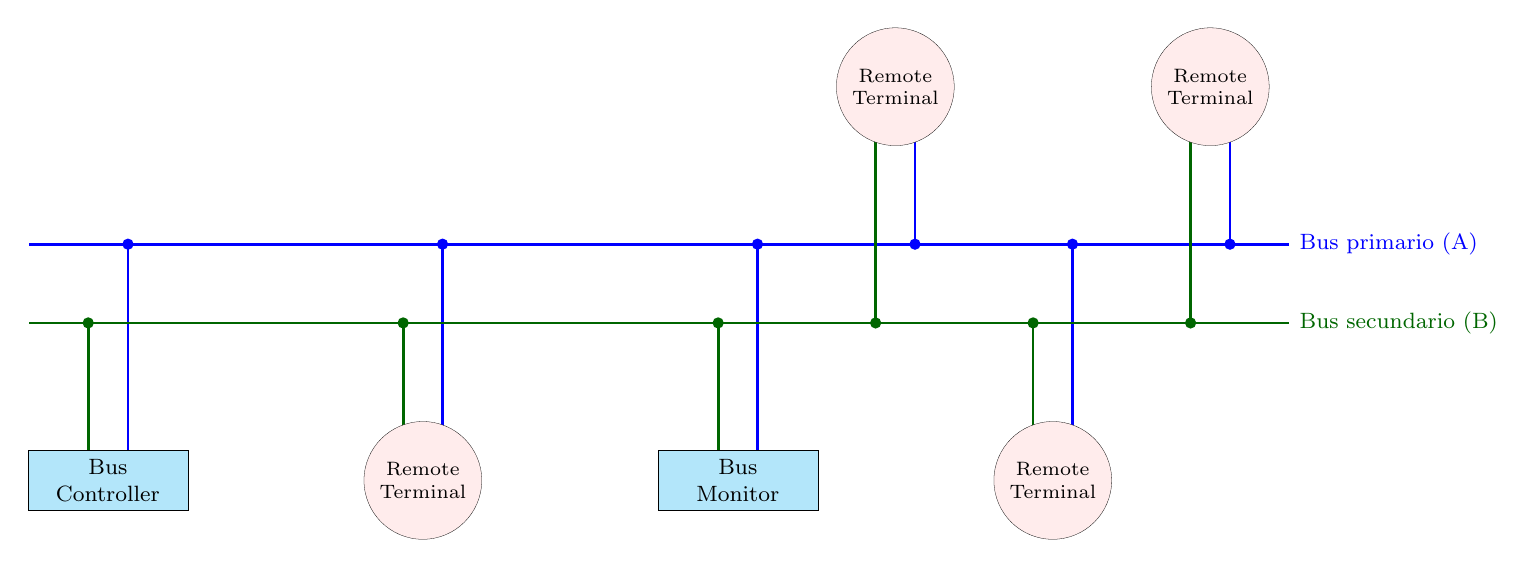
\begin{tikzpicture}[ node distance=1cm,
             conexion/.style = { circle, 
                                                 minimum size = 3 ,
                                              draw,
												fill ,
											inner sep=0 ,
                                                },
				font = \footnotesize , 
               Transmisor/.style ={ fill=cyan!30 , 
                          draw,
                          line width= 0.1 , 
						text width=1.8cm,
						align = center
                        } ,
               Receptor/.style ={  font = \scriptsize, 
						circle ,
                          fill=pink!30 , 
                          draw,
%						text width=1.2cm,
						align = center ,
                          line width= 0.1 , 
                        } ,
                     ]

% grilla
%  \draw[ green!50!black] (0,0) grid (20,10) ;

% Bus primario
\draw[line width=1, blue]  (0 , 4) -- +(16 , 0) node[above, right] {Bus primario (A)}
                       (1.255 , 4 ) node[conexion ] {} -- +(0 , -3) 
                       (5.25 , 4 ) node[conexion ] {} -- +(0 , -3) 
                       (9.25 , 4 ) node[conexion ] {} -- +(0 , -3)
                        (11.25 , 4 ) node[conexion ] {} -- +(0 , 2)
                       (13.25 , 4 ) node[conexion ] {} -- +(0 , -3) 
                       (15.25 , 4 ) node[conexion ] {} -- +(0 , 2) 
;

% Bus secundario
\draw[line width=1, green!40!black]  (0 , 3) -- +(16 , 0) node[above, right] {Bus secundario (B)} 
                       (0.75 , 3 ) node[conexion ] {} -- +(0 , -2) 
                       (4.75 , 3 ) node[conexion ] {} -- +(0 , -2) 
                       (8.75 , 3 ) node[conexion ] {} -- +(0 , -2) 
                      (10.75 , 3 ) node[conexion ] {} -- +(0 ,  3)
                      (12.75 , 3 ) node[conexion ] {} -- +(0 ,  -2)
                      (14.75 , 3 ) node[conexion ] {} -- +(0 ,  3)
;

% Elementos del bus
\draw ( 1 ,1 ) node[Transmisor] (BS) {Bus \\Controller} 
            +( 4 , 0 ) node[Receptor] (RT1) {Remote \\Terminal} 
            +( 8 , 0 ) node[Transmisor] (BM) {Bus \\ Monitor} 
            +( 10 , 5 ) node[Receptor] (RT2) {Remote \\Terminal} 
            +( 12 , 0 ) node[Receptor] (RT3) {Remote \\Terminal} 
            +( 14 , 5 ) node[Receptor] (RT4) {Remote \\Terminal} 
;





\end{tikzpicture}
%}
  \caption{Arquitectura de MIL-STD-1553, adaptado de \protect\cite{MIL-1553-tutorial}}
  \label{fig:01.MIL.1553.componentes}
\end{figure}



\subsubsection{STANAG 3838}
\label{sec:01.02.STANAG.3838}

\begin{myboxAmarillo}{STANAG}
  El STANdardization AGreement (STANAG, Acuerdo de Normalización) de
  la OTAN (Organización del Tratado del Atlántico Norte) definen
  procesos, procedimientos, términos y condiciones de equipamiento o
  procedimientos y técnicas militares comunes entre los países
  miembros de dicha alianza.
\end{myboxAmarillo}


El protocolo MIL-STD-1553 
fué adoptado por la OTAN como STANAG 3838 empleando el método de transmisión bidireccional por una sola línea  de 16 bits. Es redundante porque emplea dos buses y dos controladores de bus. Su velocidad de transmisión es de 1Mb/seg.

\subsubsection{STANAG 3910 }
\label{sec:01.02.STANAG3910 }

Es un protocolo de bus de alta velocidad de 16 bit bajo STANAG 3838 o control equivalente mediante fibra óptica. Se emplea principalmente para uso en sistemas de aviónica y que permite aumentar un bus de datos STANAG 3838 o MIL-STD-1553B de 1 Mb/seg a un bus de datos de alta velocidad de 20 Mb/seg denominado canal HS mediante, entre otros elementos, el uso de fibra óptica..

El bus STANAG 3838 / MIL-STD-1553B en una implementación de STANAG 3910 se denomina canal de baja velocidad (LS) y emplea canales de cobre. 

Ambos canales o cualquiera de ellos pueden tener redundancia múltiple y emplear medios eléctricos u ópticos.

\subsubsection{CSDB y ASCB}
\label{sec:01.02.CSDB+ASCB}

Son protocolos patentados de Collins (CSDB) y Honeywell (ASCB). 
Estos sistemas se utilizan a menudo en pequeñas empresas y aviones privados de aviación general. 

CSDB es un bus unidireccional que permite la conexión de hasta diez receptores y un transmisor. El estándar admite velocidades de datos de 12,5 kbps y 50 kbps. 

ASCB es un bus bidireccional controlado centralmente. Una configuración básica comprende un controlador de bus único y dos buses aislados, cada uno de los cuales puede admitir hasta 48 dispositivos.

\subsubsection{FDDI}
\label{sec:01.02.FDDI}

La Interfaz de Datos Distribuidos por Fibra (FDDI) fue desarrollada originalmente por Boeing para su uso en el avión Boeing 777. 

FDDI es una red de área local (LAN) basada en una topología de anillo de token dual. Los datos en cada anillo fluyen en direcciones opuestas. La velocidad de datos es de 100 Mbps y los datos se codifican en cuadros. 
CDDI (Interfaz de Datos Distribuidos de Cobre) y SDDI (Interfaz de Datos Distribuidos de Par Trenzado Blindado) son estándares de bus de red similares empleando como medios físicos cables de cobre y par trenzado blindado. 
El formato de datos es NRZI, formato de datos similar a NRZ, pero en el cual un cambio en el nivel de voltaje de línea indica un 1 lógico y ningún cambio indica un 0 lógico. 
%Por razones de costo y para reducir el número y la complejidad de los estándares de red utilizados en sus aeronaves avión, Boeing ahora planea reemplazar el sistema en el 777 con un ethernet de cobre de 10 Mbps menos costoso.
